\Aufgabe{Umsetzung in Excel}{
\begin{enumerate}
    \item Setze die Diagramme aus der vorherigen Aufgabe in einer neuen Tabellendatei um.
    \item Überlege dir einen sinnvollen Aufbau für die Tabelle und hebe auch diesmal wieder den Typ (Eingabe, berechneter Wert, Beschriftung) der Zelle (z.B. farbig) hervor. 
    \item Achte darauf, dass auch die Zwischenergebnisse wie in den Datenflussdiagrammen in der Tabelle angezeigt werden.
\end{enumerate}  

Beschreibe deinen Ansatz grob:

\LoesungLine{
\begin{itemize}
    \item Möglichkeit 1: Einfach untereinander Eingaben und berechnete Werte etwa in Reihenfolge des 'Auftretens' 
    \item Möglichkeit 2: Strukturell am DFD orientiert, wird ähnlich einer Pyramide
    \item weitere Möglichkeiten: \dots
\end{itemize}

}{3}

Zeichne eine grobe Skizze deiner Tabelle:

\LoesungKaro{
    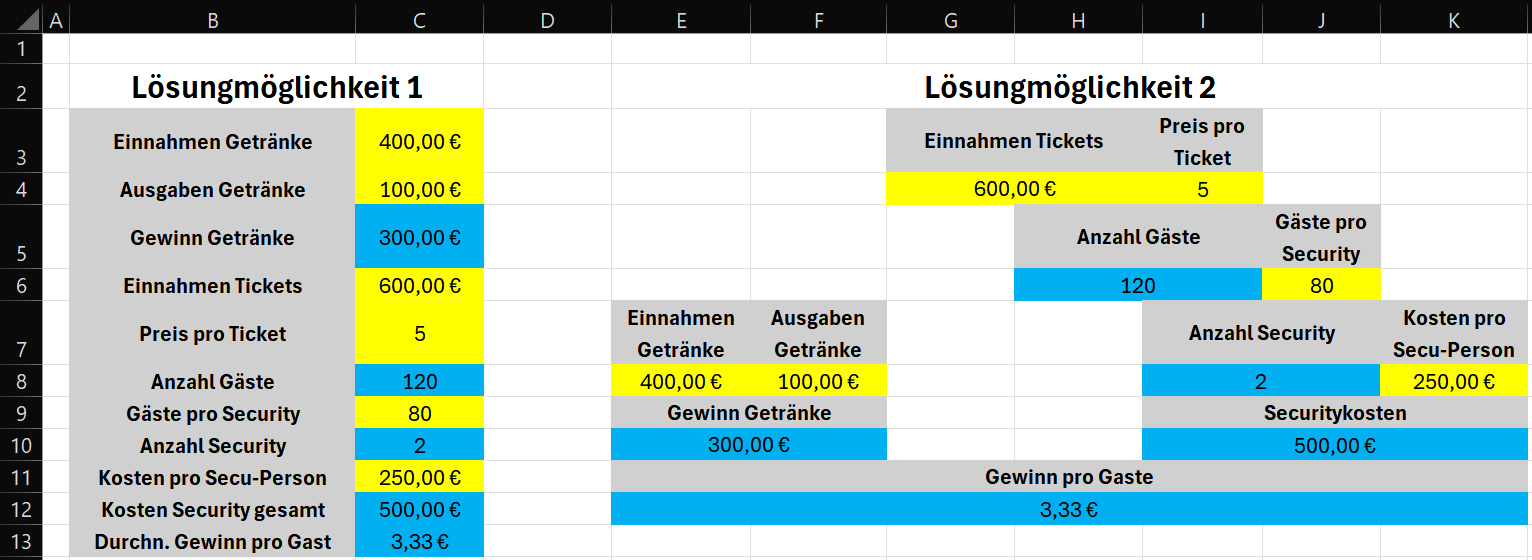
\includegraphics[width=\textwidth]{_Aufgaben/img/dfd_to_excel.png}
}{30}
}